% !TEX root = ../main.tex
\section{Risk sharing (risikodeling)}\label{thr:risk-sharing}

\paragraph{Definisjon.} \emph{Risk sharing} betegner hvordan eksogen utfallsrisiko -- variansen $\sigma^{2}$ i $Q=\alpha e+\mu$ -- fordeles mellom prinsipalen og agenten gjennom valg av kontraktsparametrene $W_0$ og $\beta$. Pareto-effisient risikodeling alene tilsier at den minst risikoaverse parten skal bære risikoen; men sammen med insentivproblemet gir dette en grunnleggende \emph{insentiv-risiko-trade-off}. [SLIDE]

\subsection*{Forklaring}

Med kontrakten $W=W_0+\beta Q$ blir variansen i agentens lønn $\mathrm{Var}[W]=\beta^{2}\sigma^{2}$. Agenten er typisk risikoavers fordi en stor andel av hennes formue og humankapital er bundet til virksomheten -- hun kan ikke diversifisere bort firmaspesifikk risiko. Prinsipalen (aksjonærer i børsnotert selskap) er derimot \emph{tilnærmet risikonøytral på marginen}, fordi hun holder en diversifisert portefølje og firmaspesifikk støy ($\mu$) er idiosynkratisk -- den ``vaskes ut'' over mange selskaper (CAPM-intuisjon). [SLIDE/BOK]

\textbf{First-best risikodeling.} Hvis innsats $e$ kunne observeres direkte og kontraherbart, ville Pareto-optimal risikodeling være at \emph{agenten får fast lønn} -- prinsipalen bærer all $\mu$-risikoen. Innsats håndteres som en kontraktsklausul: ``lever $e=e^{*}$ eller bli avskjediget''. Dette er \thref{costless-contracting}{costless contracting}-benchmark. [BOK]

\textbf{Second-best.} I virkeligheten er $e$ ikke observerbart (\thref{moral-hazard}{moral hazard}). For å vri innsats må noe av $Q$-risikoen legges på agenten ($\beta>0$). Da må prinsipalen betale en \emph{risikopremie} for at agenten skal delta:
\[
\text{risikopremie}\;\approx\;\tfrac{r}{2}\,\beta^{2}\,\sigma^{2}.
\]
Risikopremien er en \emph{deadweight cost} -- en av komponentene i \thref{agency-costs}{agency costs} (residual loss og den delen av bonding-/monitoring-strukturen som risikopremien finansierer). [BOK]

\textbf{Trade-offen.} I optimum balanseres marginal insentivgevinst (mer $e$) mot marginal risikokostnad (mer risikopremie):
\[
\underbrace{\alpha\cdot\frac{\partial e^{*}}{\partial \beta}}_{\text{insentivgevinst}}\;=\;\underbrace{r\,\beta\,\sigma^{2}}_{\text{marginal risikopremie}}.
\]
Dette gir $\beta^{*}<1$ -- agenten får \emph{noe} risiko, men ikke alt. Se \thref{optimal-effort-model}{optimal effort-modellen, modell B}. [BOK]

\subsection*{Kjerneforutsetninger}
\begin{itemize}\setlength{\itemsep}{1pt}
\item Agenten er risikoavers (CARA-nytte med $r>0$); prinsipalen er risikonøytral (eller har $r_P\ll r_A$).
\item Støyen $\mu$ er eksogen og kjent fordelt, $\mathbb{E}[\mu]=0$, $\mathrm{Var}[\mu]=\sigma^{2}$.
\item Agenten har ikke tilgang til perfekte forsikringsmarkeder for firmaspesifikk risiko.
\item Lineær kontrakt -- nødvendig for at variansformelen er ren.
\item Aksjonærer kan diversifisere idiosynkratisk risiko bort.
\end{itemize}

\subsection*{Muligheter}
\begin{itemize}\setlength{\itemsep}{1pt}
\item Forklarer hvorfor de fleste ansatte har \emph{noe} fast lønn -- ren prestasjonslønn ville være ineffektiv risikodeling.
\item Forklarer hvorfor risikable bransjer (FoU, exploration, venture) ofte har \emph{lavere} $\beta$ enn man naivt skulle tro -- den eksogene risikoen er allerede høy.
\item Forklarer bruken av \thref{informativeness-principle}{informativeness}-mekanismer som filtrerer bort uforskyldt støy (relative måltall, peer-grupper, indekserte aksjeopsjoner).
\item Forklarer hvorfor entreprenører (som tar all risiko) krever \emph{høyere forventet avkastning} (risikopremien).
\item Begrunner forsikring, hold-back-bonus, bonus-bank-mekanismer som glatter ut risiko over tid.
\end{itemize}

\subsection*{Begrensninger og kritikk}
\begin{itemize}\setlength{\itemsep}{1pt}
\item Aksjonærer er ikke alltid risikonøytrale -- dominerende eier/familieaksjonær (APMM, Wallenberg, Schibsted-fundament) er mindre diversifisert og kan være risikoavers selv.
\item Forutsetter kjent og stabilt $\sigma^{2}$ -- i virkeligheten er volatilitet selv stokastisk.
\item Risikoaversjonsparameteren $r$ er notorisk vanskelig å estimere.
\item Modellen ignorerer karriere-risiko og reputasjonsrisiko som er en stor del av agentens reelle risikoeksponering.
\item Atferdseffekter: agenter overvekter sjeldne nedsider (\emph{loss aversion}) og kan oppfatte risikopremien som utilstrekkelig.
\item Selv ved $\beta=0$ er agenten ikke fullt forsikret -- hun bærer fortsatt avskjedigelsesrisiko, og denne kan være større enn lønnsrisikoen.
\end{itemize}

\subsection*{Modell / illustrasjon}

\begin{center}
\renewcommand{\arraystretch}{1.15}
\begin{tabular}{@{}p{3.8cm}p{4.2cm}p{6.0cm}@{}}
\toprule
\textbf{Scenario} & \textbf{Hvem bærer $\mu$?} & \textbf{Konsekvens} \\
\midrule
$\beta=0$ (fastlønn) & Prinsipalen & First-best risikodeling, men ingen innsats $\Rightarrow$ shirking. \\
$\beta=1$ (residual) & Agenten & First-best innsats, men ineffektiv risikodeling $\Rightarrow$ stor risikopremie. \\
$0<\beta^{*}<1$ (second-best) & Begge proporsjonalt & Pareto-optimal gitt informasjonsasymmetrien. \\
\bottomrule
\end{tabular}
\end{center}

\begin{figure}[H]
\centering
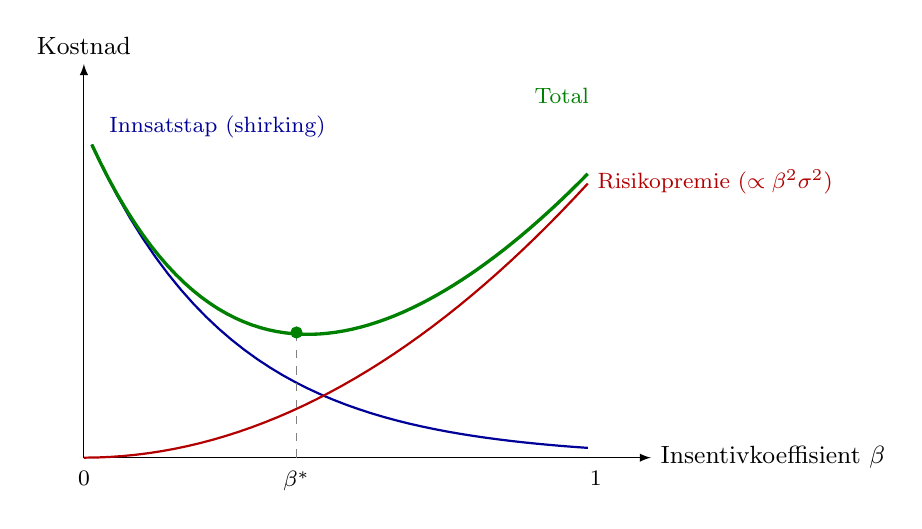
\begin{tikzpicture}[>=latex, every node/.style={font=\small}]
  % Akser
  \draw[->] (0,0) -- (7.2,0) node[right] {Insentivkoeffisient $\beta$};
  \draw[->] (0,0) -- (0,5.0) node[above] {Kostnad};
  % Markering 0 og 1 på x-aksen
  \node[below, font=\footnotesize] at (0,-0.05) {$0$};
  \node[below, font=\footnotesize] at (6.5,-0.05) {$1$};
  % Innsats-tap (synker når β øker)
  \draw[thick, blue!60!black, domain=0.1:6.4, samples=40]
    plot (\x, {4.2*exp(-0.55*\x)});
  \node[blue!60!black, font=\footnotesize, right] at (0.2,4.2) {Innsatstap (shirking)};
  % Risikopremie (stiger med β²)
  \draw[thick, red!70!black, domain=0:6.4, samples=40]
    plot (\x, {0.085*\x*\x});
  \node[red!70!black, font=\footnotesize, right] at (6.4,3.5) {Risikopremie ($\propto \beta^2 \sigma^2$)};
  % Total kostnad (sum) -- U-formet
  \draw[very thick, green!50!black, domain=0.1:6.4, samples=60]
    plot (\x, {4.2*exp(-0.55*\x) + 0.085*\x*\x});
  \node[green!50!black, font=\footnotesize, right] at (5.6,4.6) {Total};
  % β*-markering
  \draw[dashed, gray] (2.7,0) -- (2.7,1.59);
  \filldraw[green!50!black] (2.7,1.59) circle (2pt);
  \node[below, font=\bfseries\footnotesize] at (2.7,-0.05) {$\beta^*$};
\end{tikzpicture}
\caption{\textbf{Trade-offen risikodeling vs.\ insentiver.} Ved $\beta = 0$ (fastlønn): effektiv risikodeling, men maksimal shirking. Ved $\beta = 1$ (full residual claimancy): null shirking, men risikopremien koster prinsipalen $r\sigma^2/2$. Second-best $\beta^*$ minimerer summen og ligger strengt mellom 0 og 1. [SLIDE -- BSZ kap.\ 15, slide 7]}
\end{figure}

\subsection*{Eksempler}
\begin{itemize}\setlength{\itemsep}{2pt}
\item \textbf{Aksjonær vs.\ CEO i Norsk Hydro:} Aksjonær har portefølje med mange selskaper -- LME-aluminiumspris-risiko vaskes delvis ut. CEO har $\sim 80$\% av sin formue/humankapital bundet i Hydro $\Rightarrow$ risikoavers $\Rightarrow$ stor andel fast lønn + relative måltall mot peer-gruppe. [EKS]
\item \textbf{Sykehjemslege:} Output (pasientutfall) avhenger sterkt av eksogen helse hos pasienten ($\sigma^{2}$ stor). Risikodeling tilsier nesten ren fastlønn -- som er løsningen norsk offentlig sektor faktisk velger. [EKS]
\item \textbf{Hedgefond-trader (2$+$20-struktur):} Lite risikoavers, høy alfa, men $\sigma^{2}$ stor. Løsningen: ``high water mark'' og deferred compensation -- filtrerer ut deler av risiko og forhindrer asymmetrisk opp-/nedside (ekvivalent til indeksert opsjon). [EKS]
\end{itemize}

\subsection*{Kobling til søyle og andre teorier}
Søyle: \SThree\ (kontraktsdesignet legger fast risikofordelingen) med innslag av \STwo\ (måltallets støy bestemmer $\sigma^{2}$). Relaterte: \thref{optimal-effort-model}{Optimal effort-modell}, \thref{principal-agent}{Principal-agent}, \thref{incentive-coefficient}{Incentive coefficient}, \thref{fixed-vs-variable-pay}{Fast vs.\ variabel lønn}, \thref{informativeness-principle}{Informativeness-prinsippet}, \thref{moral-hazard}{Moral hazard}, \thref{agency-costs}{Agency costs}, \thref{costless-contracting}{Costless contracting} (first-best-referansen), \thref{costly-contracting}{Costly contracting}.

\paragraph{Brukt i spørsmål:} Q09, Q14, Q15.
